\section{Our methodology and Implementation}
\label{sec:implementation}


\begin{figure}[t]
{
\setlength{\belowcaptionskip}{-15pt}
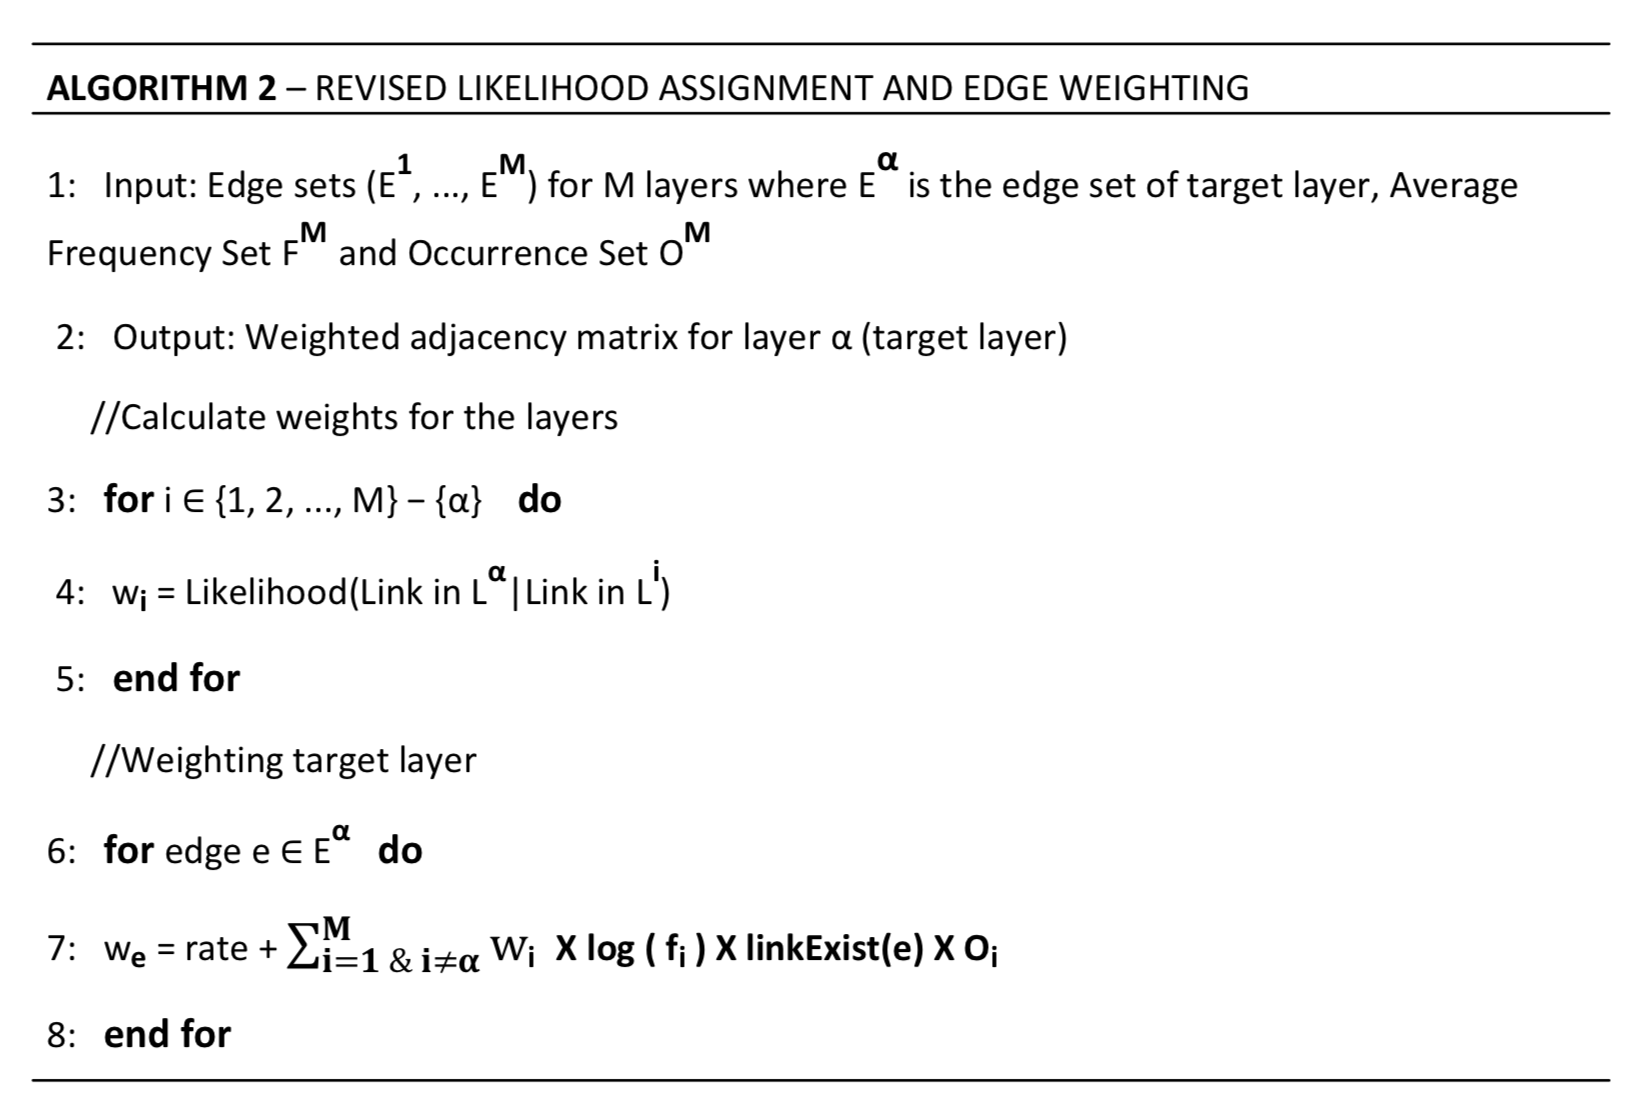
\includegraphics[width=\linewidth]{pics/algo2f.png}  
\caption{Modified version of algorithm1}
\label{fig:algo2} 
}
\end{figure}

In this paper, we perform dynamic single layer link prediction and dynamic
multiplex link prediction on the Travian dataset and conduct a comparative
analysis between the two.  In our effort to do so, we first perform dynamic
single layer link prediction at time $t'$ by calculating similarity metrics
like the Jaccard Coefficient, Preferential Attachment, Common Neighbors,
Adamic Adar, Shortest Path, and Clustering Coefficient on the aggregated
snapshots from time $t(<= t')$. We have figured all of these metrics for
performing link prediction on the attack network which also serves as the
target layer while performing dynamic multiplex link prediction.

In the case of dynamic multiplex link prediction, we form and use the trade
and message layers from the trade and message networks provided in the Travian
dataset respectively. We use these two layers to predict the links in our
target layer(Attack layer) which corresponds to the attack network in the
dataset. We have considered three variations to study the effects of different
layers on our target layer which are 1) effects of Trade layer on the Attack
layer 2) Message on Attack and 3) the combination of Message and Trade layers
on the Attack layer.

It is not a hard and fast rule to specify a particular layer as the target
layer, and also to have just one target layer. There is no limitation in the
case of number or choice when it comes to the selection of the target layer.
The same rule applies to the use of the other layers that are used to study
and calculate their influence on the attack layers.

Now to perform dynamic multiplex link prediction, we propose a new approach to
re-describe and build a new version of the Multiplex Likelihood Assignment and
Edge Weighting algorithm given above~\ref{fig:algo1}. To do this, we
reconstruct the target layer into a weighted version from its original
unweighted form by assigning weights to each edge. The weights assigned to all
of the edges to form a weighted network depends upon three factors: 1) The
interactions and connections that are common to both the target layer and the
other layers. (Ratio of the common edges between target layers and the
different layers used to predict links in the target layer) 2) The average
frequency ratio of these common edges between the target layer and the
different layers. 3) The occurrence ratio denotes, the count of the number of
times a particular edge belonging to the common edge set existed in all the
previous snapshots including the present one divided by the total number of
the snapshots. 

In our algorithm, we assign a weight to each layer based on the influence that
particular layer has on the target layer. Say for example if we want to study
the effect of the trade layer on the attack layer then we find the weight to
be assigned to the trade layer using the likelihood function where we compute
the similarity between the two layers. This similarity is nothing but the
ratio of the overlapping edges between the trade and the attack layers at the
timestep t. This similarity score assigned to each of the layers based on
their influence on the target layer is similar to the one described in
Algorithm 1~\ref{fig:algo1} and is also the first of the three factors upon
which the edge weights are dependent.

Once we have calculated the similarity scores for each of the other layers, we
now look at the second and third factors used for weighting the edges. We
compute the average frequency ratio of each common edge by taking the sum of
its frequencies in all past snapshots and dividing it by the total number of
snapshots considered. For example:- If we have to study the effect of trade
layer on the attack layer for day 3, we calculate the sum of the frequencies
of each common edge between the two layers for all the three days and divide
it by 3, to compute the average frequency ratio. Say if there are 20 common
edges between the trade and attack layer on Day 3 then for each edge in the
common edge set,we calculate the sum of the frequencies of those same 20 edges
for all the three days including the present day and divide it by 3. One
important thing to notice is if one of the edges from this common edge set is
non existent in any of the previous timesteps then for that edge the
frequency is 0 for that day. This factor gives an idea of how frequently
occurring are the edges between the two layers in all of the timesteps.

To compute the final factor for reweighing the edges we calculate an
occurrence ratio which is the count of the number of times a particular edge
from the common edge set existed in all of the timesteps divided by the total
number of timesteps. For example:- If we consider the effect of the trade
layer on the attack layer for Day 3, we already have the information regarding
the average frequency, the common edge set. We now, merely count the number of
times a particular edge from the 20 common edges (common edge set) existed in
any of the previous timesteps including the present timestep and divide it by
3(total number of timesteps in this case). This gives an idea about how often
do these common edges exist in all of the timesteps. Thus, if the edge exists
on Day 1 and Day 3 and is absent on Day 2, then the value of the count is two
by three. An important part to notice in this calculation is that the minimum
value of the count is $1/3$ as it belongs to the common edge set for the current
timestep. So even if it is not present in any of the other timesteps, the
value will be a minimum of $1/3$.

Another critical consideration taken into account other than the three factors
listed is the use of the log function on the average frequency. The reason for
doing this is to reduce the dimension of frequency ratios to the order of the
occurence ratios.
% give equal importance to both the frequency and the number of
% times the common edges exist in all of the timesteps. 
For example:- Imagine we want to study the effect of the trade layer on the
attack layer for five days and there are three edges in the common edge set.
In scenario 1) if all the three edges occur on all the days with a cumulative
frequency of $20$, then the values for average frequency ratio is $4$ and
occurence ratio is $1$, In scenario 2) if the edges occur in only $3$ days but
with a cumulative frequency of $100$, then the values of the average frequency
ratio will be $20$, and the occurence ratio is $3/5$, Thus, more importance
will be given to scenario two and a higher weight will be assigned to the
edges based on this, which is incorrect. This is because there is a higher
probability of a link formation between two nodes if they occur often and the
link between them is also frequent. Any skewness towards one of these
quantities should not be a deciding factor, and the log function on the
average frequency takes care of the same.

Apart from the proposed algorithm~\ref{fig:algo2}, we also do dynamic link
prediction in multiplex networks using  a naive strategy for completeness. To
do this,  we apply the similarity metrics on each of the layers including the
target layer at any timestep $t$ and our final  score will be an average of
the scores of all the layers.


\paragraph{Implementation. } We implemented a python toolkit using graph processing libraries such as
networkx and igraph. Experimentation was done on a standalone pc, with 16 GB
Ram and i7 processor. 


% \subsection{Our method}
% \label{sec:method}

% Say what differently are we doing to the methods 
% descibed in background~\ref{sec:background} section. 

% \subsection{Implementaiton}
% \label{sec:implementation}

% Say how did we implement our project. Describe the tool 
% and its working.